% !TEX root = ../agglo_clust_review.tex
% 
\begin{figure}
\centering

        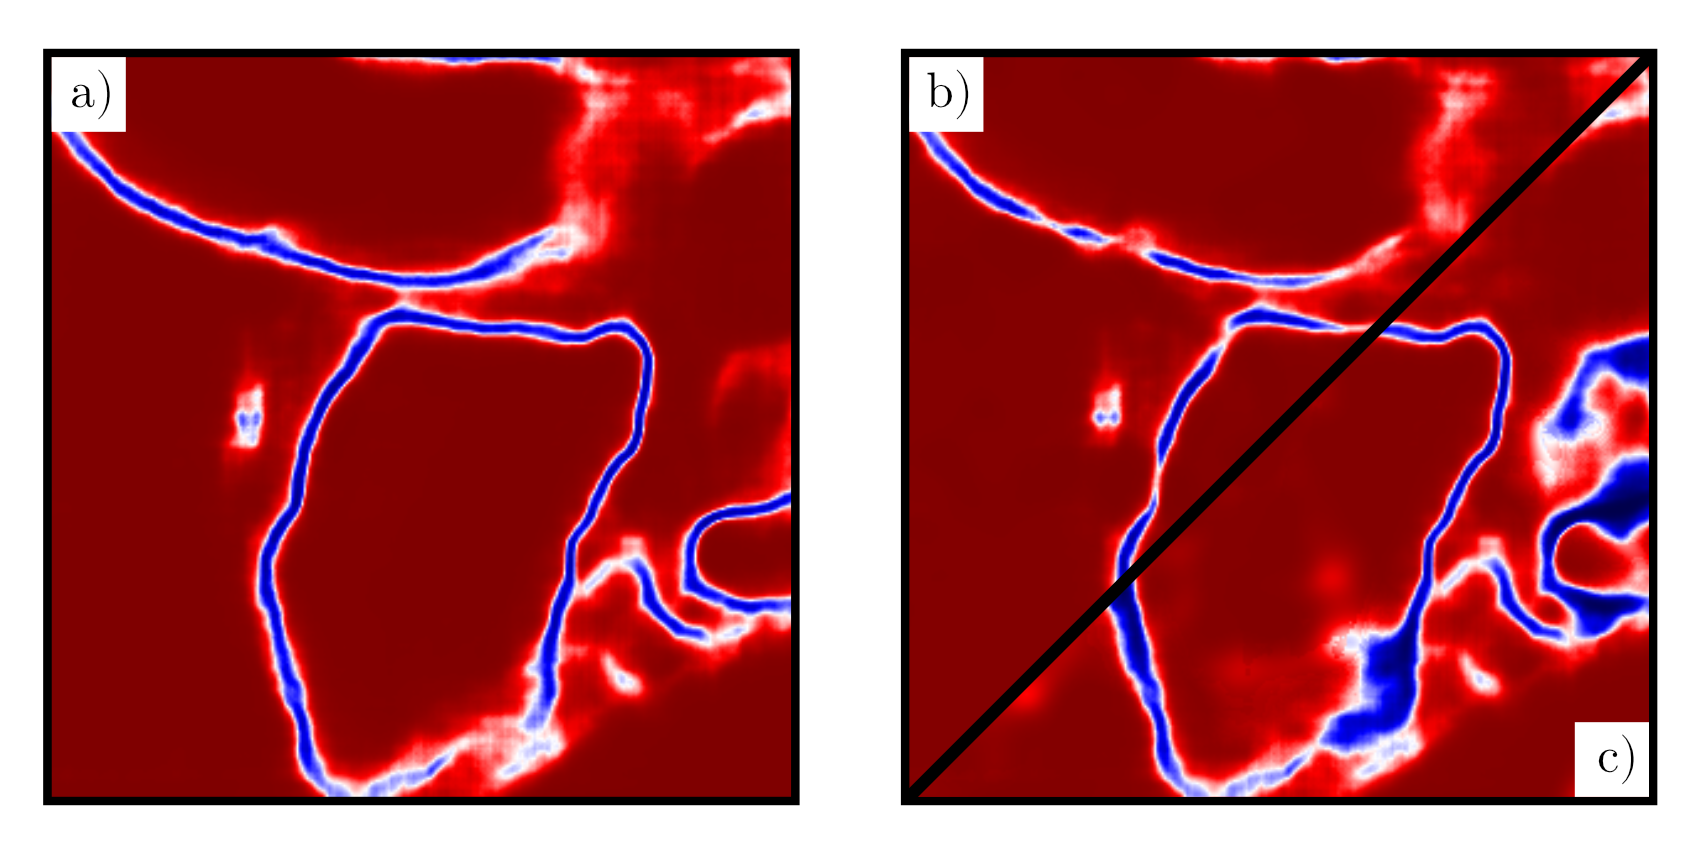
\includegraphics[width=0.48\textwidth,trim=0.1in 0.0in 0.05in 0.0in,clip]{figs/noisy_affs_comparison.png}
   
    \caption{The two figures represent the predictions of the CNN on the CREMI dataset (\UPDATE{REF}) a) without added noise, b) with the addition of the merge-biased noise defined in Eq. \ref{eq:opensimplex_noise_def} and c) with split-biased noise. The color of each pixel represents how probable it is for it to be in the same cluster with its neighboring pixel on the right (red: same cluster; blue: different ones). Adding merge-biased noise tends to create holes in the boundaries; split-biased noise add non-existing boundaries \TODO{Add colorbar? Adapt to noise defs}}
    \label{fig:noisy_affs}
\end{figure}% 

\begin{figure*}
\centering
        \begin{subfigure}[t]{0.48 \textwidth}
        \centering
        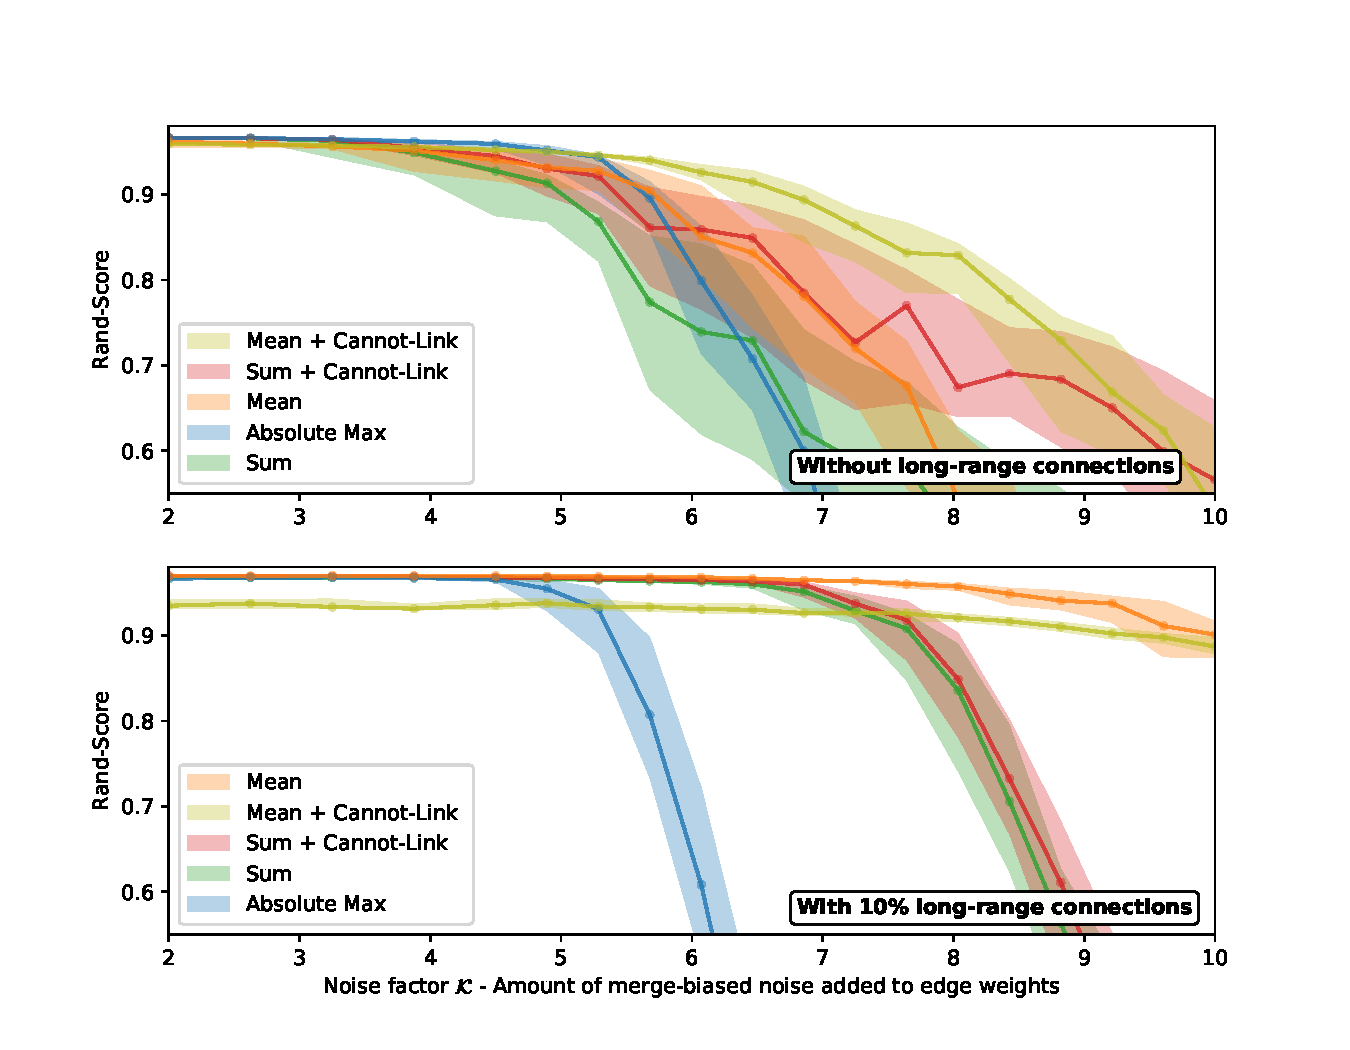
\includegraphics[width=0.98\textwidth,trim=0.35in 0.35in 0.35in 0.35in,clip]{./figs/merge_noise.pdf}

        \caption{Merge-biased opensimplex noise} \label{fig:thresh}
    \end{subfigure}%
    \begin{subfigure}[t]{0.48 \textwidth}
        \centering
        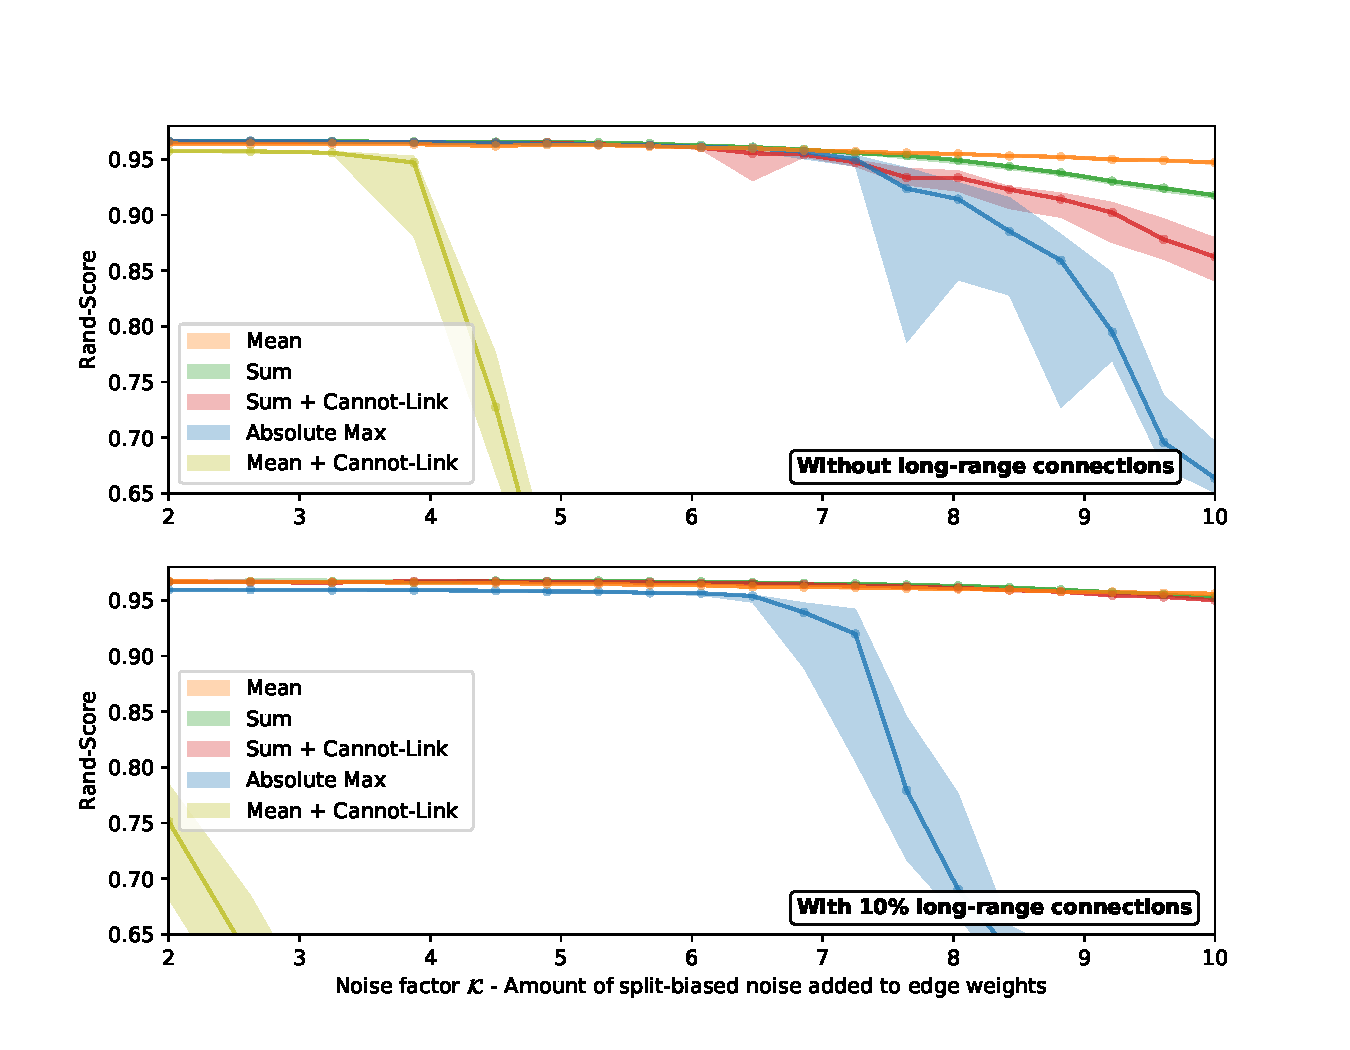
\includegraphics[width=0.98\textwidth,trim=0.29in 0.31in 0.31in 0.31in,clip]{./figs/split_noise.pdf}
        \caption{Split-biased opensimplex noise} \label{fig:ws}
    \end{subfigure}


\caption{Plot illustrating Adapted RAND scores achieved by UGACA and different update rules when noise is added to the edge weights... \TODO{Label which uses only local-neighbors and which uses long-range connections}}\label{fig:noise_plots}
\end{figure*}


\subsection{Testing the robustness of the algorithms}
 In this section we will quantitatively test the robustness of UGACA by adding noise to the edge weights of the graph and see how different choices of update rules compare.

 Among the update rules listed in Table \ref{tab:linkage-criteria}, we will focus only on \emph{sum}, \emph{arithmetic mean} and \emph{absolute maximum}, since they achieved the best scores in the results presented in Sec. \ref{sec:exp_first_comparison}. Before to present the results shown in Fig. \ref{fig:noise_merge}, we will first introduce the type of noise that was added to the edge weights.

 In the set of experiments presented in this article, edge weights are estimated \UPDATE{by using a CNN that predicts how likely two neighboring pixels are to be part of the same cluster}. Fig. \hyperref[fig:noisy_affs]{\ref*{fig:noisy_affs}a} illustrates the predictions of the CNN on the CREMI dataset for neuron segmentation. We would now like to make these predictions worse by introducing  artifacts, \UPDATE{e.g. partially deleted or added boundaries between neurons in the image}. In the field of image processing there are several ways of adding noise to an image, among which the most common are Gaussian noise or Poisson shot noise. By using these methods, the noise value of each pixel is independent of noise values of neighboring pixels, thus they are not a good choice for our application since the pixelwise predictions of a CNN are usually spatially correlated. 

 We then decided to use Perlin noise\footnote{In our experiments, we used opensimplex noise, that is a more recent open-source version of Perlin noise (\UPDATE{REF or link?})}, one of the most common gradient noises used in procedural pattern generation. This type of noise generates spatial random patterns that are locally smooth but have large and diverse variations on bigger scales. It generates values $n(x)\in[0,1]$ that were mapped to $[-\infty, \infty]$ with the Logit function, $N(x)=\mathrm{Logit}(n(x))$, and then combined with the original CNN predictions $F(x)=\mathrm{Logit}(p(x))$ in the two different following ways:
\begin{equation}
% \tilde{F}(x;\theta)=\begin{cases}
% F(x;\theta)+\mathcal{K}\cdot\max\left(N(x),0\right) & \text{if merge-biased}\\
% F(x;\theta)+\mathcal{K}\cdot\min\left(N(x),0\right) & \text{if split-biased}
% \end{cases}
\tilde{F}_{\pm}(x;\mathcal{K})=F(x)\pm\big|\mathcal{K}\cdot\max\left(\pm N(x),0\right)\big|,
\end{equation}
In this equation, $\mathcal{K}\in \mathbb{R}^+$ is a positive factor representing the amount of added noise; $\tilde{F}_{+}(x;\mathcal{K})$ represents a merge-biased modified version of the CNN predictions $F(x)$, such that the probability for two pixels to be in the same cluster is increased only if $N(x)>0$ (see Fig. \hyperref[fig:noisy_affs]{\ref*{fig:noisy_affs}b}); on the other hand, $\tilde{F}_{-}(x;\mathcal{K})$ represents a split-biased prediction with decreased probabilities only when $N(x)<0$ (Fig. \hyperref[fig:noisy_affs]{\ref*{fig:noisy_affs}c}). In the Supplementary material we provide a detailed description of the parameters used for the noise generation.

With this strategy, we randomly perturbed the CNN predictions and the edge weights only in some parts of the image. The plots in Fig. \ref{fig:noise_plots} represent the scores achieved by UGACA with different update rules depending on the amount of noise $\mathcal{K}$ added to the edge weights. 
\begin{itemize}
\item The experiments show that running UGACA on a grid graph with long-range connections always lead to better segmentations/clusterings \TODO{require def. of long range graph and long-range probability}
\item The most robust version of update rule proved to be the arithmetic mean, that achieves similar scores even when a significantly noisy edge weights.
\item The \emph{absolute maximum} update rule proposed by \cite{wolf2018mutex} provides an efficient and fast option, but it completely fails when too much noise is added.
\item The \emph{sum} update rule version was the slowest option tested, but it was not as robust as the \emph{mean} version, probably due to its tendency to grow one cluster at the time (see Sec. \ref{sec:exp_first_comparison}). Comment about MC energy (plots in Suppl. Material?)
\item On the other hand, UGACA with mean update rule and cannot-link constraints never achieves good overall scores, as we have already shown in Sec. \ref{sec:exp_first_comparison} and \UPDATE{Figure...?}, because \UPDATE{it tends to introduce too many false splits}. 
%Nevertheless, these additional experiments show that it provides an \UPDATE{almost true over-segmentation of the ground truth segmentation even with strongly merge-biased predictions}.
\end{itemize}


% \begin{equation}
% \begin{gathered}
% \tilde{p}_{\pm}(x;\theta)=\sigma(\tilde{F}_{\pm}(x;\theta))\quad \text{where}\\
% % \tilde{F}(x;\theta)=\begin{cases}
% % F(x;\theta)+\mathcal{K}\cdot\max\left(N(x),0\right) & \text{if merge-biased}\\
% % F(x;\theta)+\mathcal{K}\cdot\min\left(N(x),0\right) & \text{if split-biased}
% % \end{cases}
% \tilde{F}_{\pm}(x;\theta)=F(x;\theta)\pm\left|\mathcal{K}\cdot\max\left(\pm N(x),0\right)\right|
% \end{gathered}
% \end{equation}
